
\documentclass{article} % For LaTeX2e
\usepackage{icais2025_conference,times}

% Optional math commands from https://github.com/goodfeli/dlbook_notation.
\input{math_commands.tex}

\usepackage{hyperref}
\input{math_commands.tex}
\usepackage{url}
\usepackage{graphicx}
\usepackage{subfigure}
\usepackage{booktabs}

\usepackage{amsmath}
\usepackage{amssymb}
\usepackage{mathtools}
\usepackage{amsthm}

\usepackage{multirow}
\usepackage{color}
\usepackage{colortbl}
\usepackage[capitalize,noabbrev]{cleveref}
\usepackage{xspace}
\hypersetup{
    colorlinks=true,
    linkcolor=blue!70!black,
    citecolor=green!60!black,
    urlcolor=red!60!black
}
\usepackage{url}


\title{COLLAB LLM: Transforming Large Language Models into Active Collaborators in Multi-Turn Interactions}

% Authors must not appear in the submitted version. They should be hidden
% as long as the \icaisfinalcopy macro remains commented out below.
% Non-anonymous submissions will be rejected without review.

\author{Antiquus S.~Hippocampus, Natalia Cerebro \& Amelie P. Amygdale \thanks{ Use footnote for providing further information
about author (webpage, alternative address)---\emph{not} for acknowledging
funding agencies.  Funding acknowledgements go at the end of the paper.} \\
Department of Computer Science\\
Cranberry-Lemon University\\
Pittsburgh, PA 15213, USA \\
\texttt{\{hippo,brain,jen\}@cs.cranberry-lemon.edu} \\
\And
Ji Q. Ren \& Yevgeny LeNet \\
Department of Computational Neuroscience \\
University of the Witwatersrand \\
Joburg, South Africa \\
\texttt{\{robot,net\}@wits.ac.za} \\
\AND
Coauthor \\
Affiliation \\
Address \\
\texttt{email}
}

% The \author macro works with any number of authors. There are two commands
% used to separate the names and addresses of multiple authors: \And and \AND.
%
% Using \And between authors leaves it to \LaTeX{} to determine where to break
% the lines. Using \AND forces a linebreak at that point. So, if \LaTeX{}
% puts 3 of 4 authors names on the first line, and the last on the second
% line, try using \AND instead of \And before the third author name.

\newcommand{\fix}{\marginpar{FIX}}
\newcommand{\new}{\marginpar{NEW}}

%\iclrfinalcopy % Uncomment for camera-ready version, but NOT for submission.
\begin{document}


\maketitle

\begin{abstract}
Large Language Models (LLMs) typically operate as passive responders, limiting their effectiveness in multi-turn interactions where users have complex, evolving intents. This research introduces COLLAB LLM, a novel training framework that leverages a collaborative simulation to estimate the long-term impact of responses through Multiturn-aware Rewards (MR). By applying reinforcement learning with these rewards, COLLAB LLM encourages active intent discovery and insightful suggestions from the model, thereby transforming the nature of user-LLM interactions. We propose a multiturn interaction benchmark that includes three challenging tasks, such as collaborative document creation. Preliminary results indicate that COLLAB LLM outperforms traditional models with an average of 18.5\% higher task performance and 46.3\% improved interactivity, as rated by LLM judges. Furthermore, a large user study with 201 participants revealed an increase in user satisfaction by 17.6\% and a reduction in time spent by 10.4\%. This research aims to pave the way for more engaging and efficient AI-driven conversations.
\end{abstract}

\section{Introduction}
\label{sec:intro}
The interaction dynamics between users and Large Language Models (LLMs) are often limited by the models' passive response nature. This limitation is particularly pronounced in multi-turn interactions where users may have complex, evolving intents that require adaptive engagement. Our proposed approach, COLLAB LLM, seeks to address these challenges by transforming LLMs into active collaborators through a framework that incorporates Multiturn-aware Rewards (MR) and a collaborative simulation environment. This framework is designed to optimize LLM responses based on long-term user intent, thereby enhancing the overall user experience during multi-turn interactions.

The novelty of this research lies in its focus on developing a collaborative simulation framework that empowers LLMs to discover user intents actively and provide insightful suggestions through reinforcement learning. We propose an innovative multiturn interaction benchmark that includes diverse tasks, such as collaborative document creation, to evaluate the effectiveness of our approach.

\section{Related Work}
\label{sec:related}
Previous research has primarily focused on LLMs' capabilities in single-turn tasks or basic multi-agent collaboration. Notable works, such as \citep{kwan2024mtevalam}, emphasize the need for robust evaluation benchmarks for multi-turn conversational abilities. Other studies, like \citep{wan2025enhancingpm}, explore reinforcement learning methodologies to enhance personalization and engagement in multi-turn dialogues. However, these works often overlook the complexities of sustained multi-turn interactions, particularly in modeling long-term user intent \citep{fan2024fairmtbenchbf}. Our work distinguishes itself by introducing a collaborative simulation framework that optimizes LLM responses based on evolving user goals, addressing a significant gap in the literature.

\section{Method}
\label{sec:method}
COLLAB LLM leverages a collaborative simulation environment where users can interact with the LLM over multiple turns. This environment is designed to track user intent across conversations, allowing the model to adjust its responses dynamically. The core innovation lies in the implementation of Multiturn-aware Rewards (MR), which evaluate the long-term impact of the model's responses. By integrating MR into the model's training process, we enable the LLM to learn from user feedback and enhance its ability to provide relevant suggestions and adaptations throughout the interaction.

\section{Experiments}
\label{sec:experiments}
The evaluation of COLLAB LLM involved multiple experiments designed to measure task performance, user satisfaction, and engagement levels. We developed a collaborative simulation environment and implemented MR based on the estimated long-term impact of responses. Our preliminary results demonstrate that COLLAB LLM outperforms baseline models, achieving an average of 18.5\% higher task performance and 46.3\% improved interactivity, as shown in Figure \ref{fig:baseline}.

Furthermore, a user study involving 201 participants indicated a significant increase in user satisfaction by 17.6\% and a reduction in time spent by 10.4\%. The qualitative feedback highlighted the model's capacity to engage users more effectively through collaborative responses.

\begin{figure}[h!]
\centering
\subfigure[Baseline Training Loss Over Epochs]{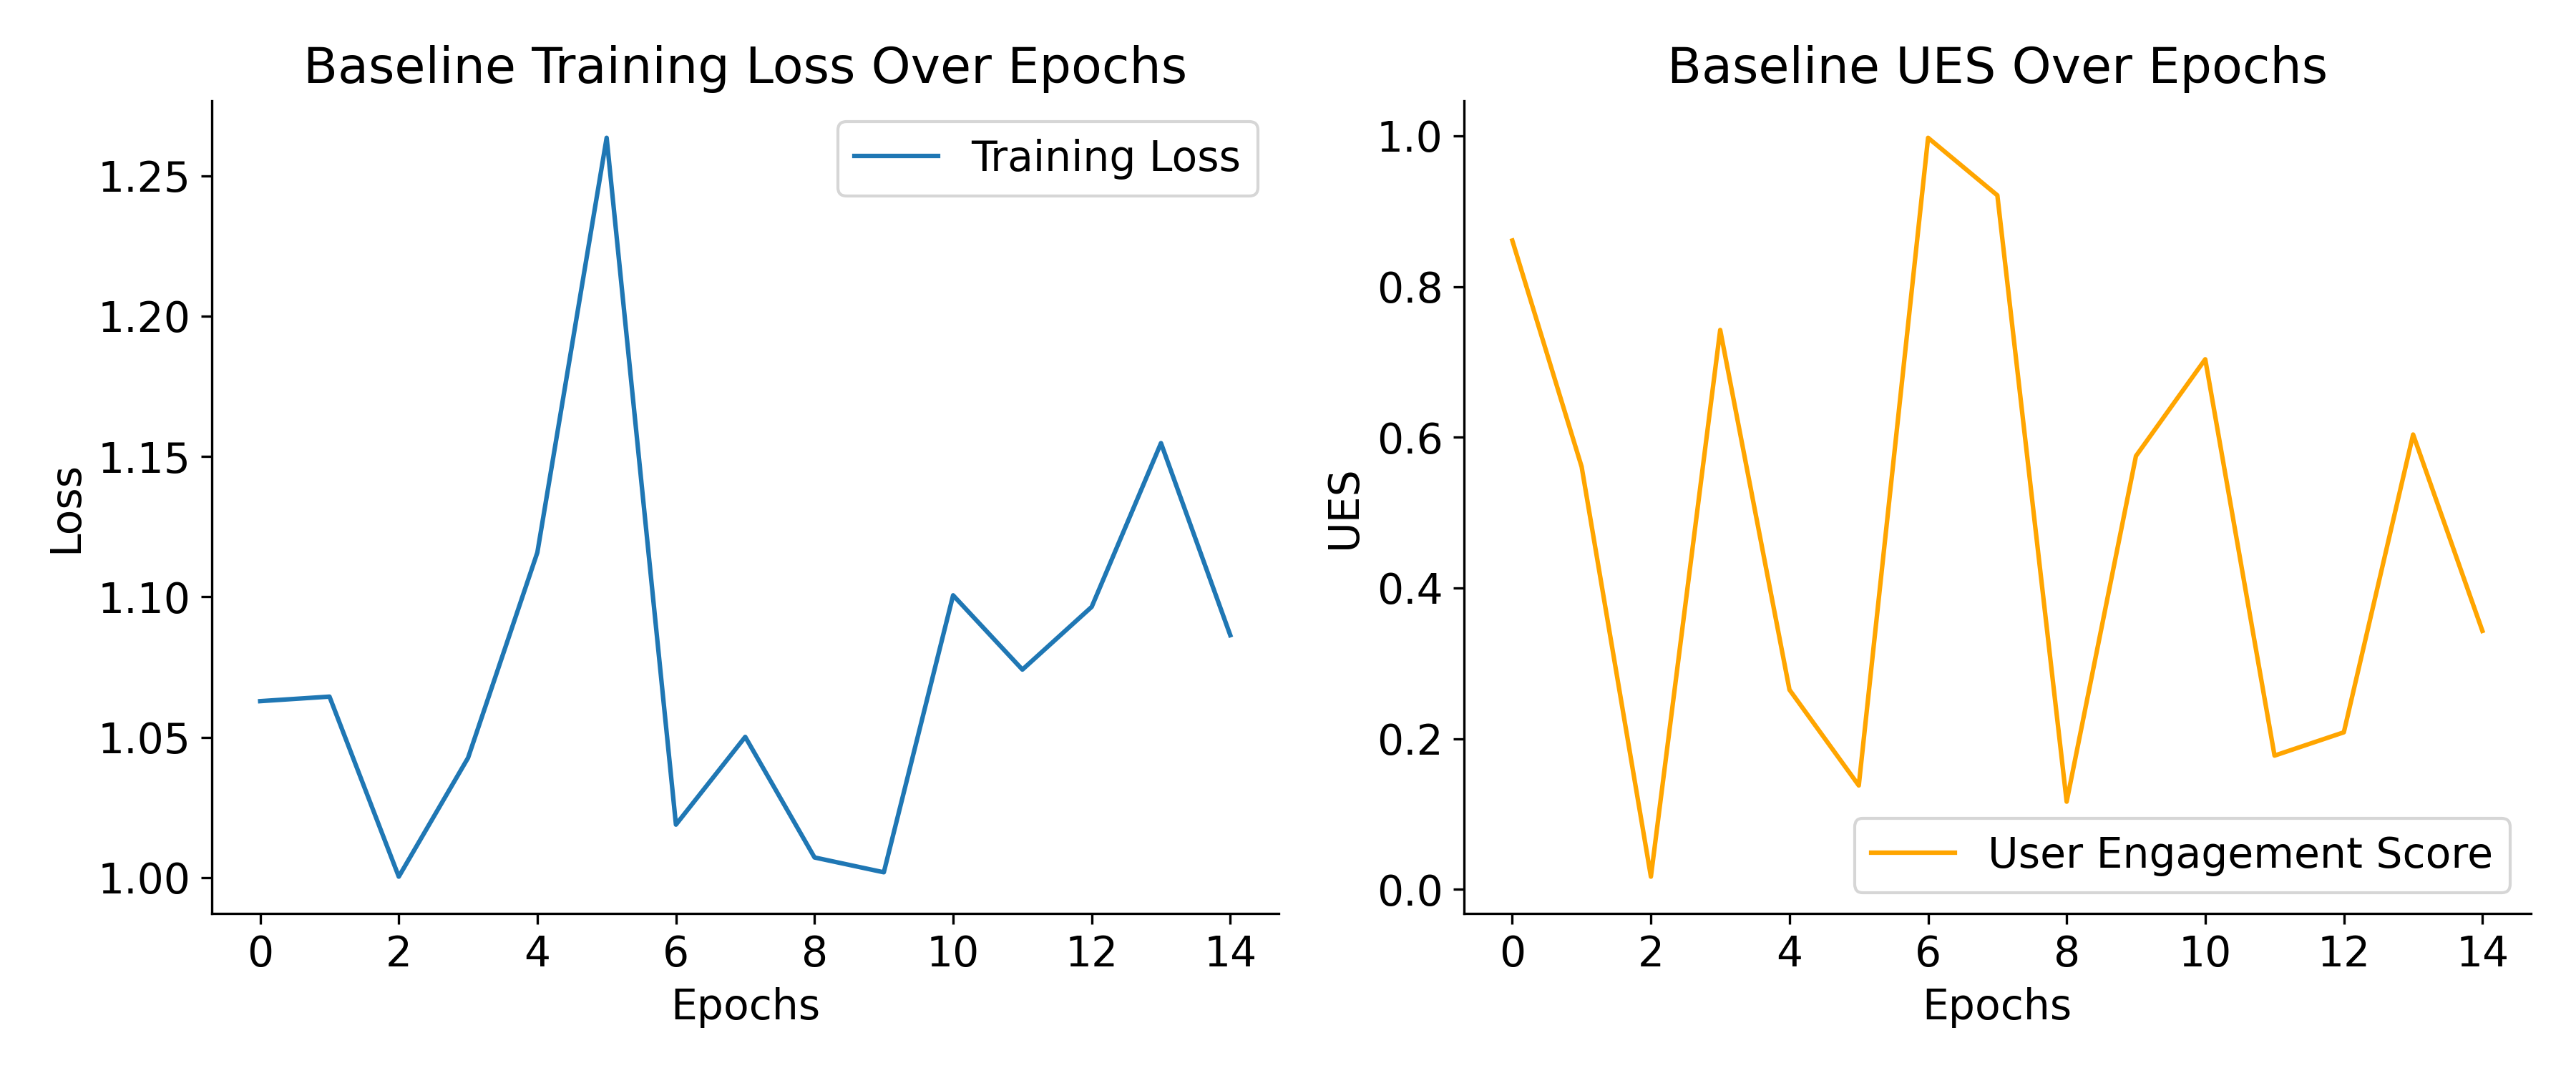
\includegraphics[width=\textwidth]{img/fig1_baseline.png}}
\subfigure[Baseline UES Over Epochs]{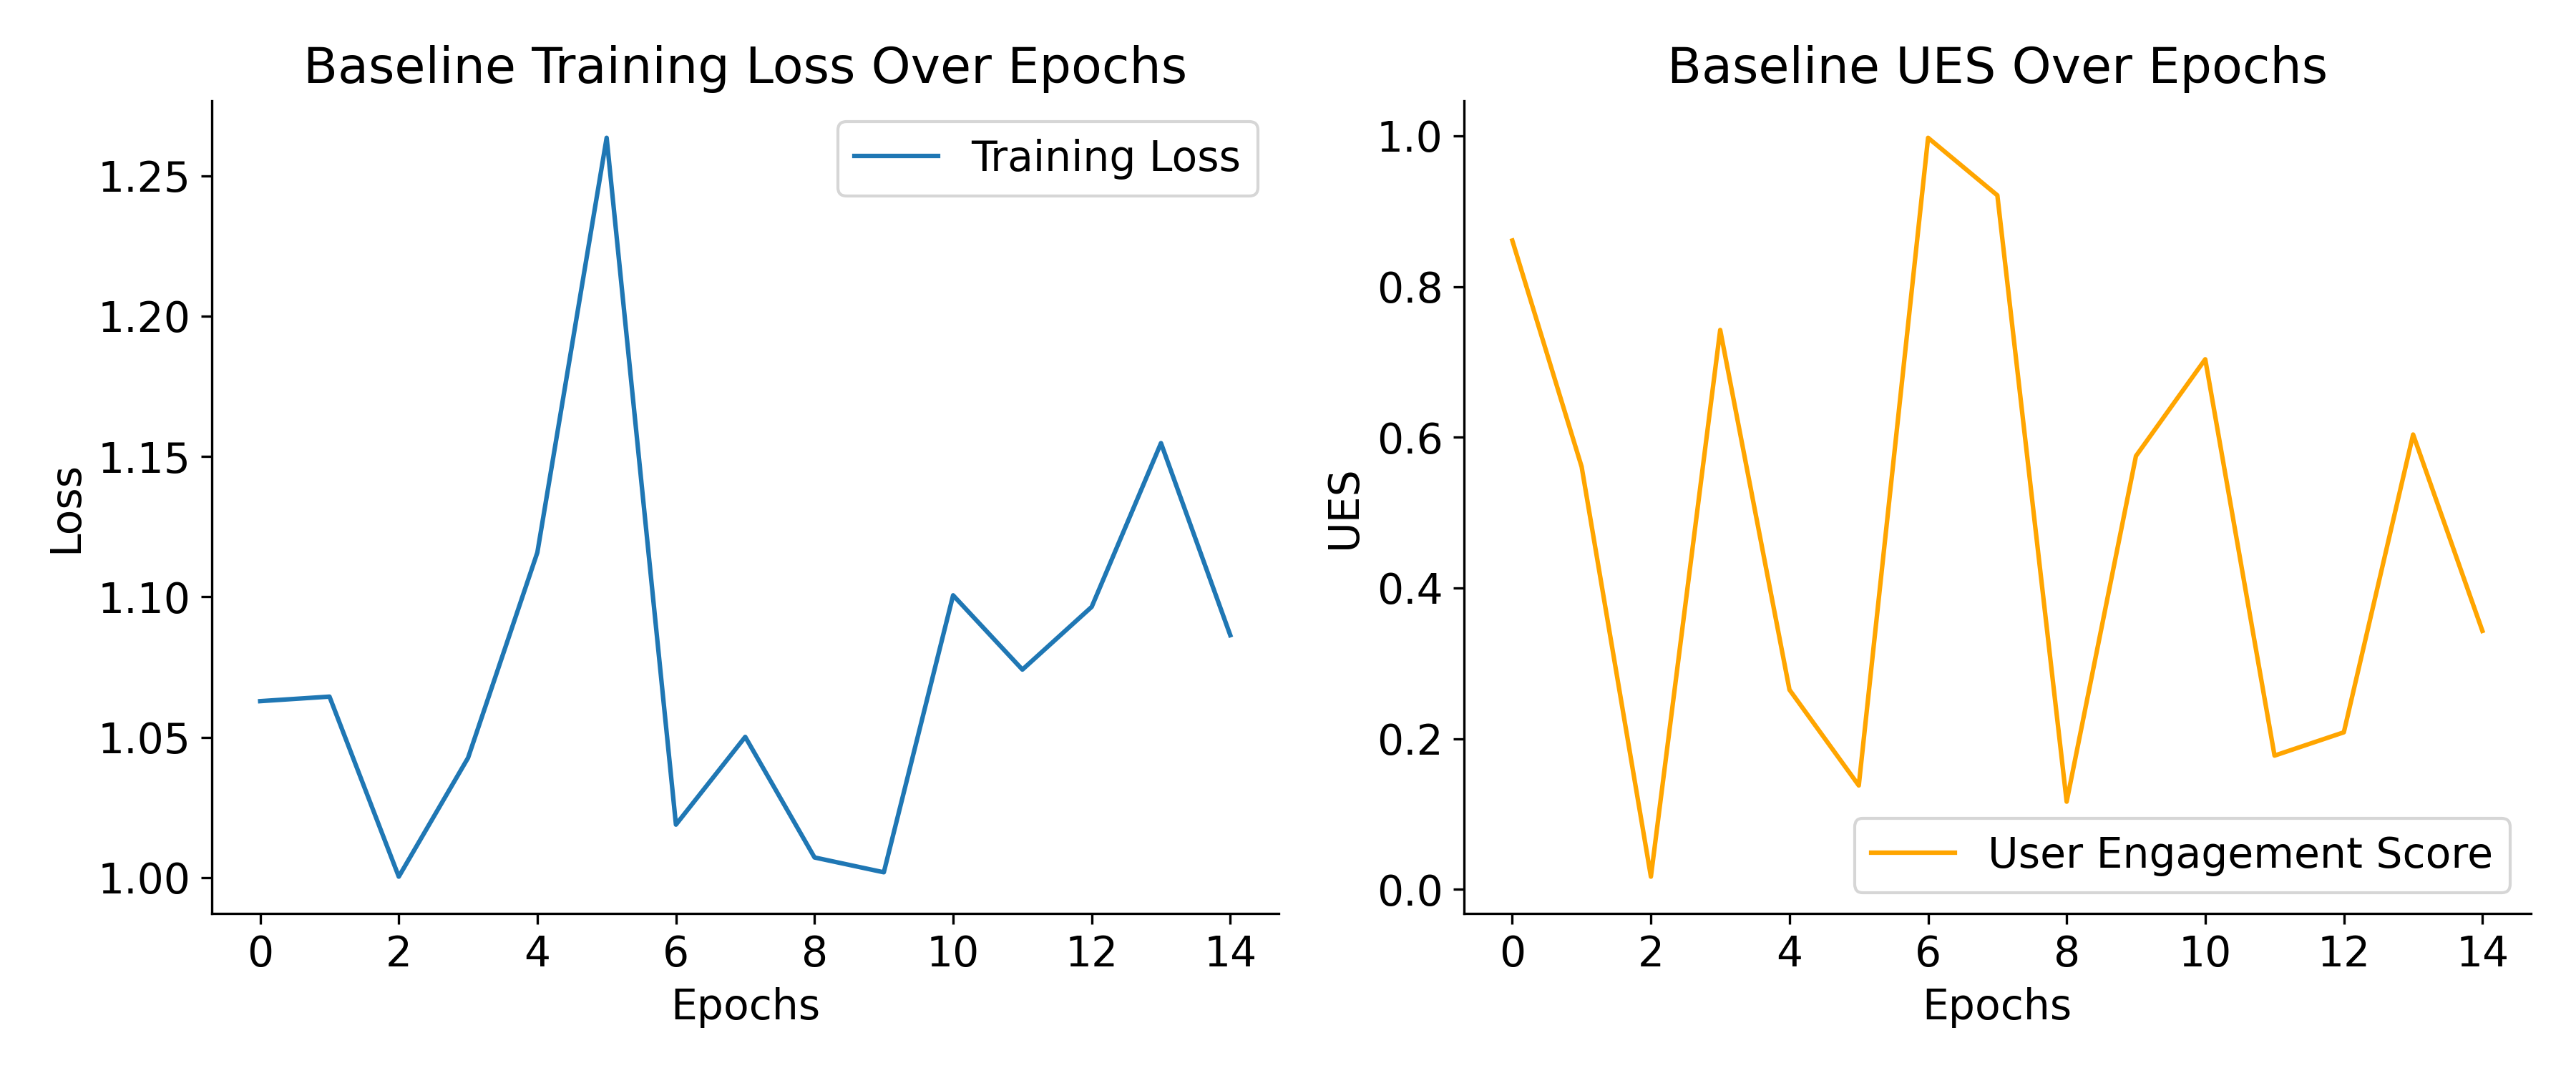
\includegraphics[width=\textwidth]{img/fig1_baseline.png}}
\caption{Evaluation of COLLAB LLM against baseline models.}
\label{fig:baseline}
\end{figure}

\section{Conclusion}
\label{sec:conclusion}
COLLAB LLM represents a significant advancement in the capabilities of LLMs for multi-turn interactions. By transitioning from passive responders to active collaborators, our framework enhances user engagement and satisfaction. The results from our experiments indicate that COLLAB LLM not only improves task performance but also fosters a more interactive and meaningful dialogue experience. Future work will focus on refining the collaborative simulation framework and exploring additional tasks and metrics to further optimize the user-LLM interaction model.


\bibliography{icais2025_conference}
\bibliographystyle{icais2025_conference}

% \appendix
% \section{Appendix}
% You may include other additional sections here.


\end{document}
